\chapter{\label{cha:context} Technical Background}

This chapter thoroughly discusses the two central systems the project is concerned with: Apache Ranger and OpenMetadat. It will also briefly cover related items, such as building a local debugging harness, Java practices for developing large, distributed and extensible frameworks and dependency management. As mentioned in Section \ref{sec:project_goal}, this chapter aims to present itself as an introduction to the inner working of Apache Ranger and methodologies for expanding its suite of interoperable services.  

\section{OpenMetadata}

The OpenMetadata system is written in multiple languages (Java, Python and Typescript); its source code is packaged as an Apache Maven project with submodules representing different parts of the framework. The system is composed of the following elements:

\begin{itemize}
    \item \textbf{Metadata Store} - PostgreSQL or MySQL database that stores metadata information;
    \item \textbf{Search Engine} - Elasticsearch engine for fast queries of metadata information;
    \item \textbf{Standard Schemas} - definitions for types and entities used across all the components, defined using JSON Schemas \cite{foundationOfJsonSchemaPezoa2016} (module \mintinline[breaklines,breakafter=.:]{java}{org.open-metadata:openmetadata-spec});  
    \item \textbf{Metadata Service} - web service, written in Java, based on the Dropwizard framework \cite{dropwizardTech}, that governs access to metadata and provides the system's API (module \mintinline[breaklines,breakafter=.:-]{java}{org.open-metadata:openmetadata-service});
    \item \textbf{User Interface} - single page application, written Typescript, using the React framework \cite{reactTech} (module \mintinline{java}{org.open-metadata:openmetadata-ui});
    \item \textbf{Ingestion Framework} - Python package that crawls data stores to gather and report metadata (PiPy package \mintinline{text}{openmetadata-ingestion}).
\end{itemize}

Figure \ref{fig:openmetadata_arch} represents a compact architectural diagram of the OpenMetadata system. Components marked with dotted lines represent external services. 

\begin{figure}
    \centering
    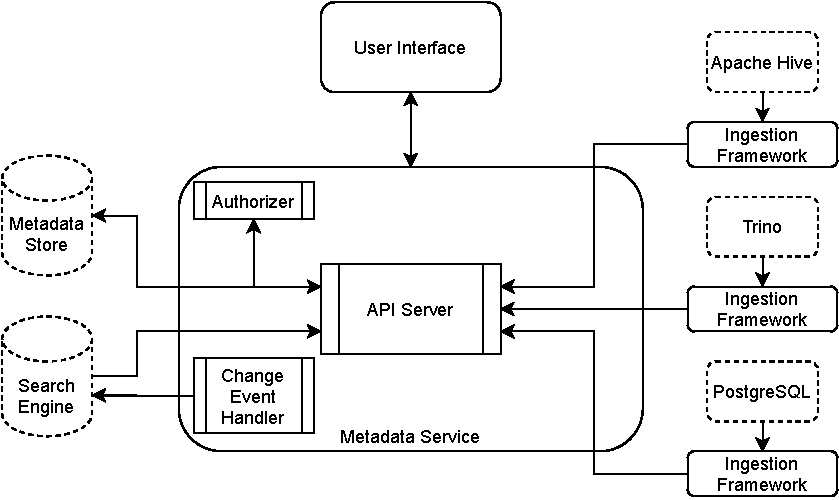
\includegraphics[width=0.8\textwidth]{chapters/tech_background/figures/openmetadata-arch.pdf}
    \caption{Architectural diagram of the OpenMetadata system.}
    \label{fig:openmetadata_arch}
\end{figure}

\subsection{User Interface}

\begin{figure}
    \centering
    
    \subfloat[\centering \label{fig:openmetadata_sample_data_table} Page showing metadata of a sample table in OpenMetadata.]{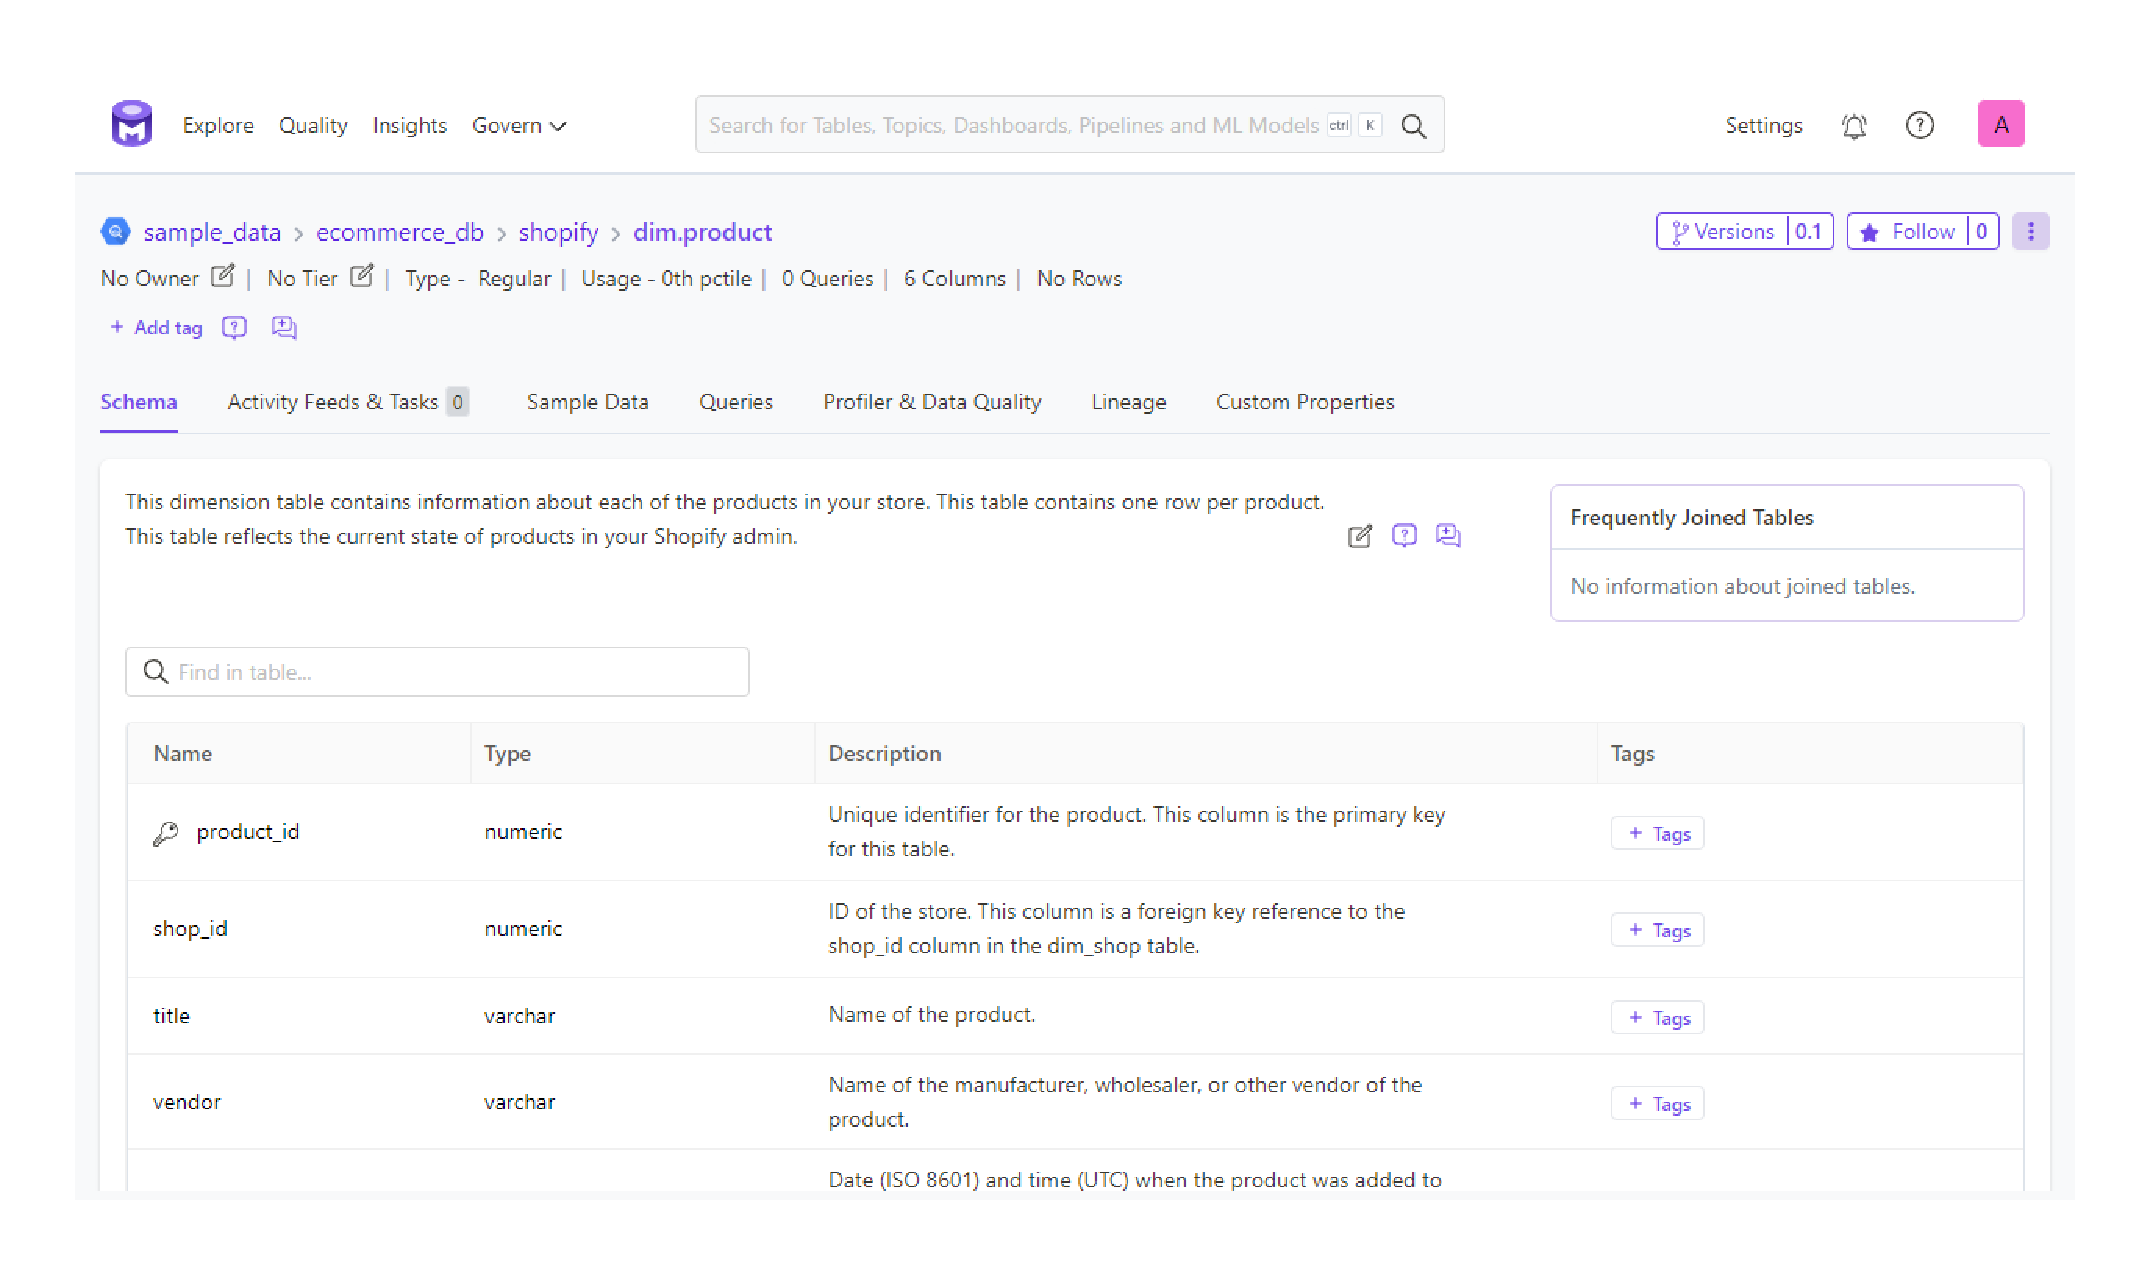
\includegraphics[width=\textwidth]{chapters/tech_background/figures/openmetadata_sample_data_table.pdf}} 

    \qquad

    \subfloat[\centering \label{fig:openmetadata_sample_data_explore} Search page from OpenMetadata.]{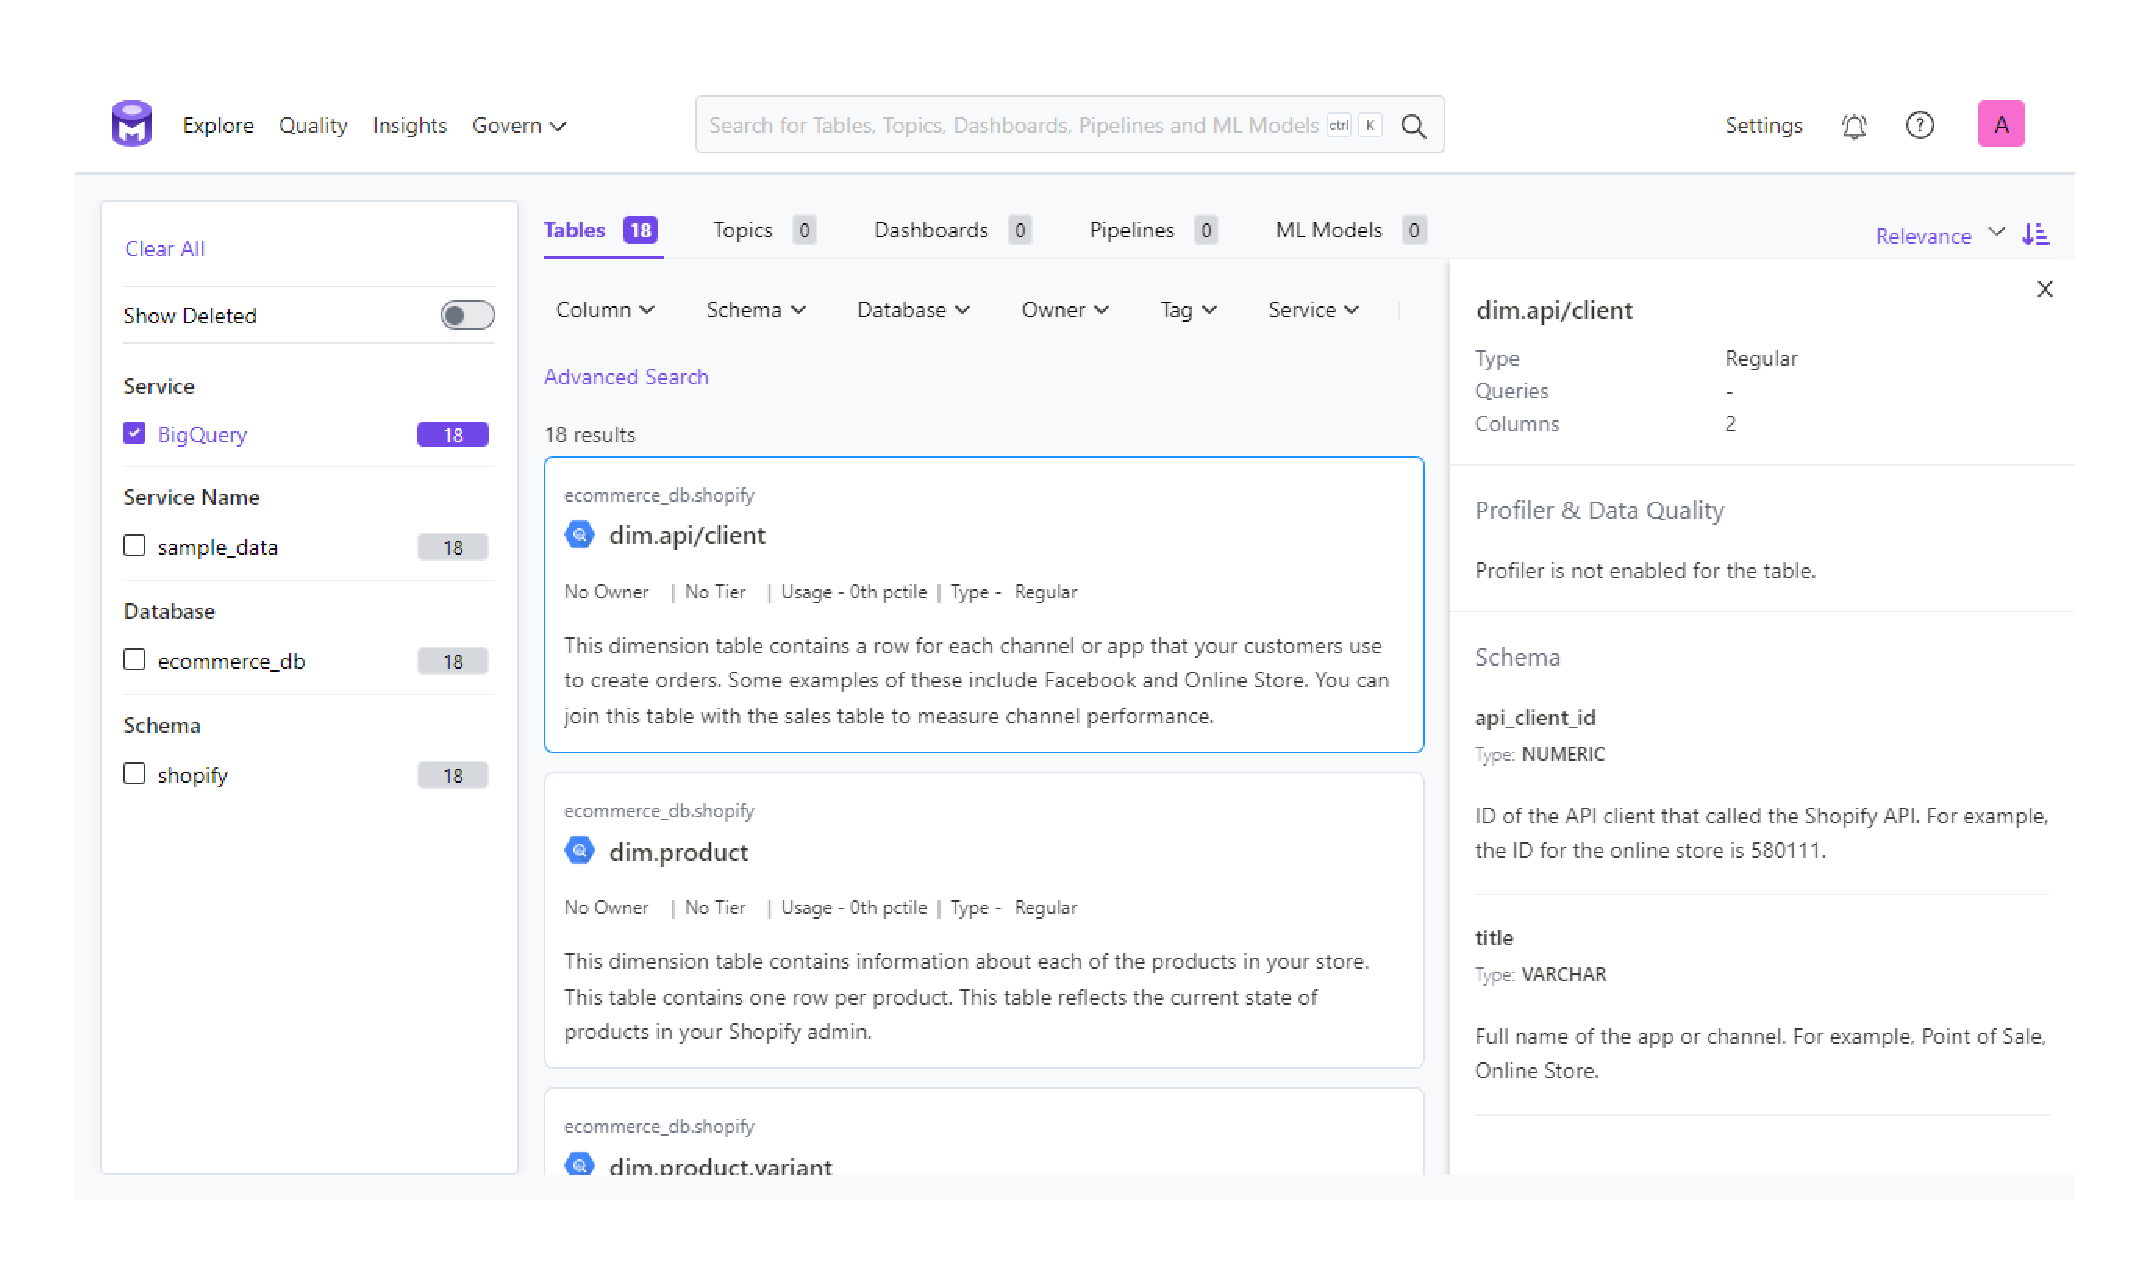
\includegraphics[width=\textwidth]{chapters/tech_background/figures/openmetadata_sample_data_explore.pdf}}
    
    \caption{Sample screenshots from the OpenMetadata user interface.}
\end{figure}

The user interface is how data analysts, data scientists and domain experts interact with the OpenMetadata system to search for resources, view metadata, edit descriptions, tag datasets, and collaborate.

Figure \ref{fig:openmetadata_sample_data_table} shows the information page of the \mintinline{text}{shopify>dim.product} tables ingested from a Google Big Query database, containing the fully quantified name of the resource, the schema of the table, the type of each column, description, owner information and associated tags, among others. This page also provides functionality for editing user-modifiable metadata about the resource, like the description and tags.

Figure \ref{fig:openmetadata_sample_data_explore} shows the system's search functionality. The left-hand side panel contains facet-style filters used to remove unwanted results quickly. The right-hand side panel has a preview of the selected resource. The central panel lists all the results of the search along with more filters for specific properties of tables and a complex query builder under the "Advanced Search" button.

Functionally, the user interface uses the publicly exposed APIs of the Metadata Service and an authentication provider to handle logins. The build process dynamically generates Typescript interfaces from the Standard Schemas provided as JSON schemas which are then available in the user interface source code.

\subsection{Metadata Service}

The Metadata Service is the system's core, governing all reading, updating, creating and deleting metadata. The system treats all resources (e.g., databases, tables, tags, users, dashboards, workflows) as entities, sharing a common interface, defined in the Standard Schema as \mintinline{java}{EntityInterface}. The \mintinline{java}{EntityReference} type provides links to other entities without storing their full representation. Entities can have extensions, storing additional information that can optionally be fetched if needed, and two entities can have a relationship, which can further store information about their relationship.

The API provides a common pattern of endpoints for CRUD operations on all entity types, and certain entities also support specialized operations. We list examples of common requests below:

\begin{itemize}
    \item \mintinline{text}{GET /api/v1/<entityType>/<id>} - retrieves an Entity instance by ID;
    \item \mintinline{text}{GET /api/v1/<entityType>/name/<fullyQualifiedName>} - retrieves an Entity instance using its fully qualified name;
    \item \mintinline{text}{PUT /api/v1/<entityType>} - updates an existing Entity instance or creates a new one.
\end{itemize}

\subsection{Access Control Mechanism}

The Metadata Service handles access control for all operations that interact with entities through an \mintinline{java}{Authorizer} interface, which checks the subject's permission to apply an action to a resource. The included implementation of this interface (aptly named \mintinline{java}{DefaultAuthorizer}) uses a role-based access control system established on the NIST "Flat RBAC" model \cite{nistRBAC2000Sandhu, buildingAccessControlForOpenMetadata2022Mathew}, which is very similar to the mechanism employed by Apache Ranger, with some essential differences that will be discussed later. 

The model defines the following components:

\begin{itemize}
    \item \textbf{Rules} - an object comprised of a set of resource types, a set of access types, an effect, which can be either allowed or denied, and a condition, written in the Spring Expression Language (SpEL);
    \item \textbf{Policy} - a set of rules;
    \item \textbf{Role} - a set of policies where each policy can be enabled or disabled.
\end{itemize}

Users are assigned roles case-by-case or through their teams and departments. The user interface handles all configuration, and the Metadata Store stores the rules, policies and roles. Conditional rules enable contextual matching, affecting only resources which meet criteria (e.g., the \mintinline{java}{isOwner()} directive matches only resources of which the current user is the owner). 

\subsection{Downfalls of the included authorization system and the need for Apache Ranger}

The access control system included with OpenMetadata was designed to provide an adequate solution for small to medium-sized organizations, where migrating users and departments to OpenMetadata is manageable with no automation and the level of access granularity need not be too precise.

We claim that the provided system is inadequate for large organizations, with particular attention to organizations that implement company-wide access control systems looking for precise access control of their metadata and wish to integrate OpenMetadata with existing infrastructure.

\begin{enumerate}

    \item \textbf{Granularity of resources in rules.} Access control rules can be applied to all resources of a particular type but not to specific resources; thus, constraining access on a resource-by-resource basis is impossible. For example, a rule can allow reading of all table resources, but not specifically of the \mintinline[breaklines, breakbefore=>]{java}{sample_data>ecommerce_db>shopify>dim.product} table. Condition rules mimic this behaviour but are limited and challenging to manage and, thus, not a suitable alternative.

    \item \textbf{Integration with Active Directory.} Active Directory systems are, for many organizations, the central database of users and groups and often serve as a common language for integrating with proprietary or legacy software; thus, they need to be a part of the access control framework. OpenMetadata could adapt to these systems by mimicking a subset of the resource structures in an Active Directory employing its internal representation of users and teams. Still, this process is not officially supported and is likely prone to desynchronization issues.

    \item \textbf{Governance of access control and administration.} Finally, the security of such a system is only as good as the access control rules that govern it. OpenMetadata manages these through the UI and handles permissions to view or modify rules and policies using the authorization system; thus, it suffers from the issues outlined in point 1.

\end{enumerate}

These deficiencies motivate integrating OpenMetadata with Apache Ranger, as the latter is an industry-tested tool that aims to tackle these issues.

\section{Active Directory and Lightweight Directory Access Protocol}

TODO: Add background here.

\section{\label{sec:tech_background_apache_ranger} Apache Ranger}

Terms commonly used from here on out are defined as follows:

\begin{itemize}
    \item \textbf{Service definition} - a definition for a type of service (e.g., Hive, HDFS, HBase) in JSON format;
    \item \textbf{Service} - a connection to an external process using an Apache Ranger plugin to govern access control, comprised of configuration and a list of policies. Configuration is commonly composed of connection parameters, allowing Ranger to communicate with the external process;
    \item \textbf{External user} - an account in the organisation and managed using Active Directory (e.g., LDAP) or Unix-compatible user and group systems. Users have a unique username and are members of a set of groups, which may represent the user's department or permissions;
    \item \textbf{Role} - a shorthand for a specific set of users, groups and other roles that exist only in the Ranger Security Admin Service (it is not part of the organisation's Active Directory);
    \item \textbf{Resource} - any data, application, or service that needs to be protected and managed by the access control system. Resources can take many forms, such as databases, tables, columns, HDFS paths, Hive queries, Kafka topics, and Elasticsearch topics;
    \item \textbf{Access type} - a way a user can interact with a resource. Common access types are view, edit, create and delete; 
    \item \textbf{Policy} - a rule that describes what access types certain users are permitted to use on a set of resources with a common pattern.
\end{itemize}

\begin{figure}
    \centering
    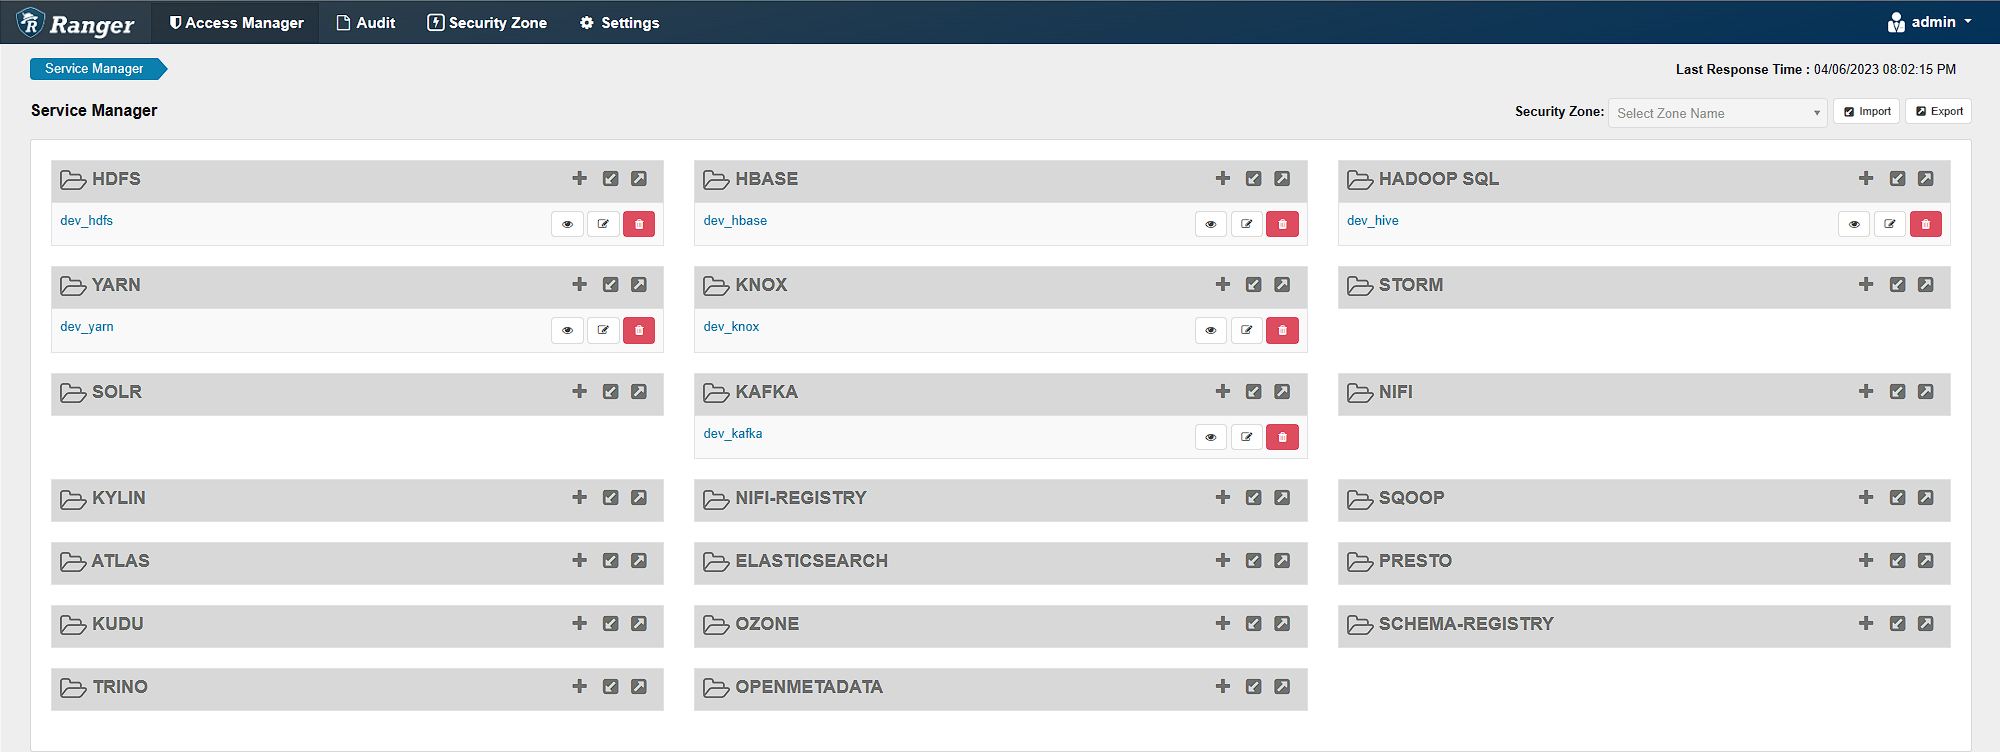
\includegraphics[width=\textwidth]{chapters/tech_background/figures/ranger-admin.png}
    \caption{Landing page for Apache Ranger user interface, showing sample services.}
    \label{fig:ranger-admin}
\end{figure}

\begin{figure}
    \centering
    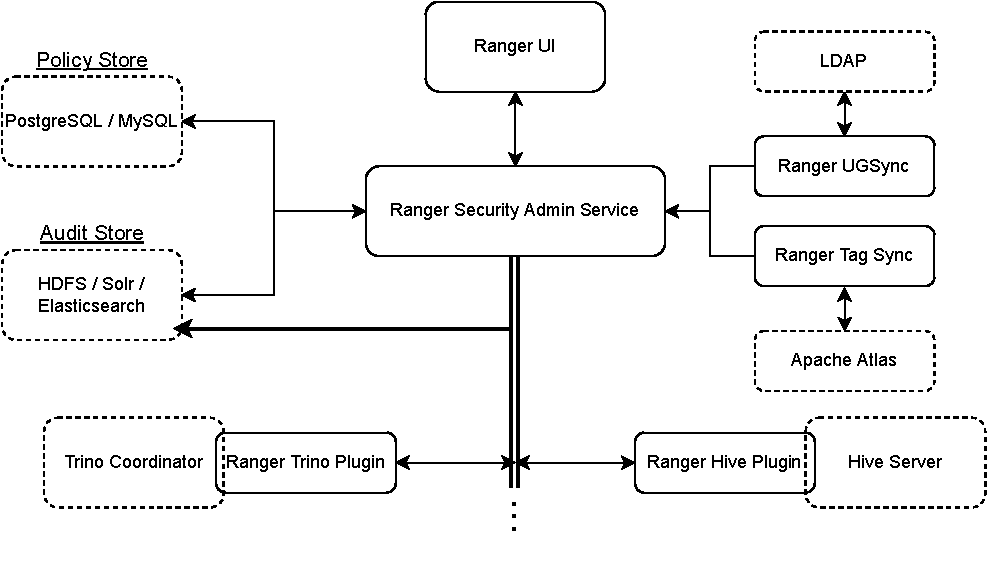
\includegraphics[width=0.8\textwidth]{chapters/tech_background/figures/ranger-arch.pdf}
    \caption{Architectural diagram of the Apache Ranger system.}
    \label{fig:rager_arch}
\end{figure}

All the core components of the Apache Ranger framework are written in Java, originally developed using Java 8, but forwards-compatible with Java 11, and the user interface is written in JavaScript. Apache Maven \cite{apacheMavenTech} handles the project's structure and build. It is split into multiple modules, each concerned with different framework parts. We will be looking at \mintinline{java}{security-admin} (also referred to as the security admin service), \mintinline{java}{ugsync} (a short name for user and group sync) and plugins with their respective shims (e.g., \mintinline{java}{plugin-trino} and \mintinline{java}{range-trino-plugin-shim}). Figure \ref{fig:rager_arch} shows an architectural diagram of Apache Ranger's primary components, with full boxes representing first-party components and dashed boxes representing external services.

The \mintinline{java}{security-admin}, along with the user interface, is the heart of the system and the place where admins will define and connect services and manage access policies, security zones and user roles. Figure \ref{fig:ranger-admin} shows the landing page of the user interface, where various demo services have been added.

Figure \ref{fig:ranger_hive} shows the eight default policies created for the \mintinline{java}{dev_hive} service, and Figure \ref{fig:ranger_hive_poly} shows the details of the \mintinline[breaklines]{java}{all - database, table, column} policy, which is defined for resources that follow pattern \mintinline[breaklines]{java}{{database="*", table="*", column="*"}}, which can be read as "all columns, in all tables, in all databases". The policy allows the \mintinline{java}{hive} user to do a subset of all actions. It enables the owner of the resource (\mintinline{java}{{OWNER}} is a macro that is replaced with the owner of the resources at evaluation time) to do all actions on these resources.

The \mintinline{java}{ugservice} is an asynchronous process that monitors an Active Directory or a Unix-compatible user and group systems and populates the security admin service's repository of external users and groups.

\begin{figure}
    \centering
    \subfloat[\centering \label{fig:ranger_hive} All policies created for the \mintinline{java}{dev_hive} Hive service.]{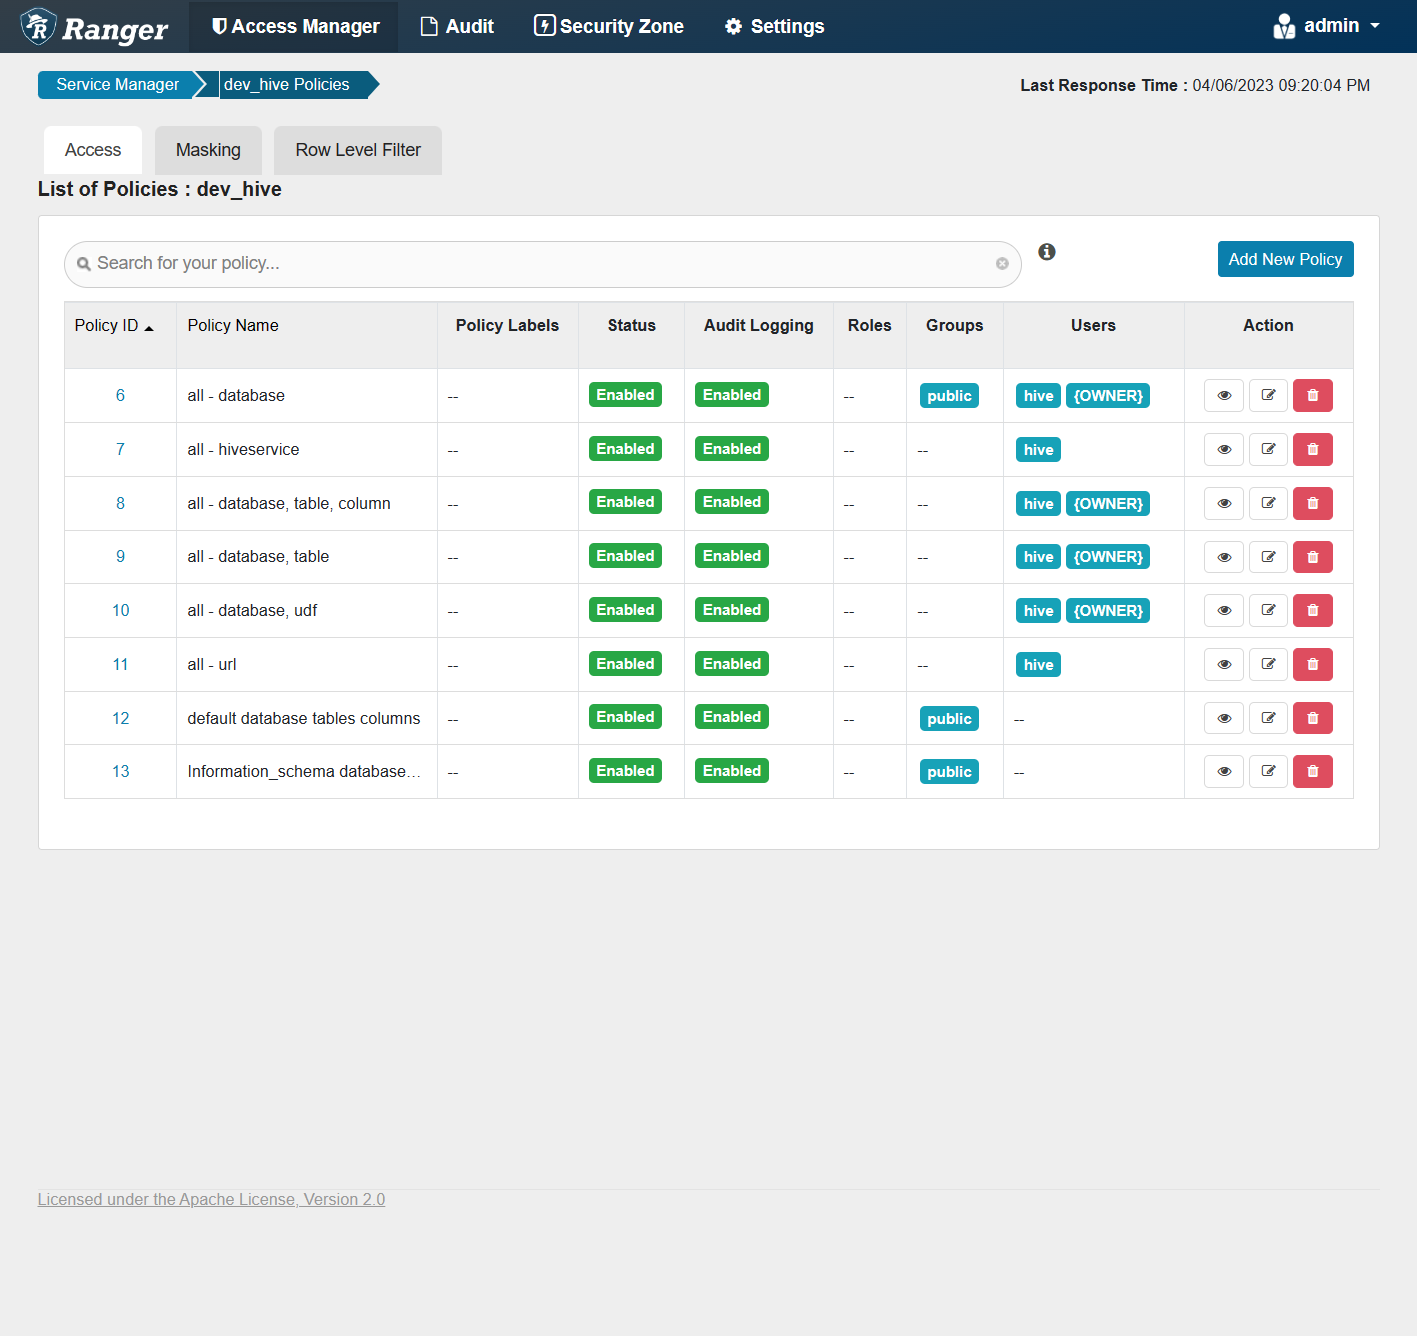
\includegraphics[width=0.65\textwidth]{chapters/tech_background/figures/ranger_hive.png}}
    \qquad
    \subfloat[\centering \label{fig:ranger_hive_poly} The \mintinline{java}{all - database, table, column} policy defined for the Hive service.]{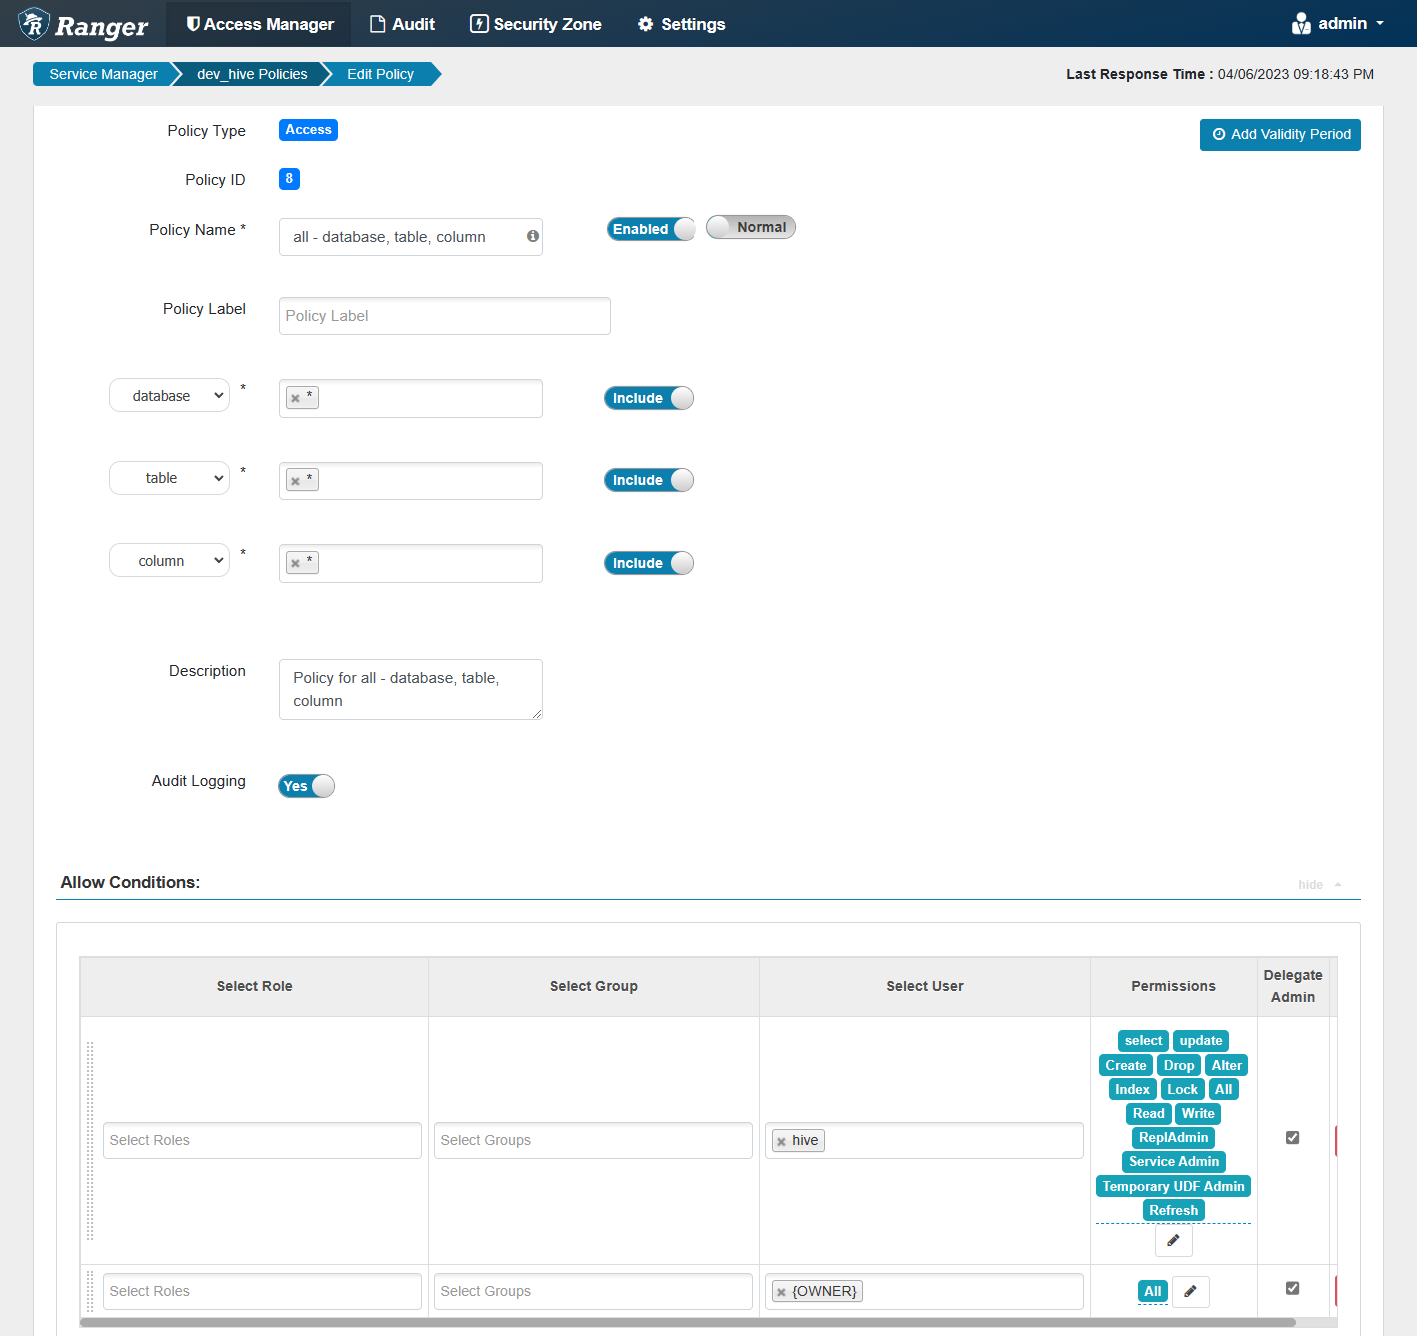
\includegraphics[width=0.65\textwidth]{chapters/tech_background/figures/ranger_hive_poly.png}}
    \caption{Sample configuration for a Hive service in Apache Ranger.}
    \label{fig:ranger_hive_details}
\end{figure}

\subsection{\label{sec:plugins_for_apache_ranger} Plugins for Apache Ranger}

All services defined in Apache Ranger are treated as plugins, sharing a common interface independent of what the external Service is doing. A plugin has two components:

\begin{itemize}
    \item \textbf{A service type definition} - also referred to as the \mintinline{text}{serviceDef.json} file. The file can be added as part of the source code in the folder \mintinline[breaklines, breakafter=/]{java}{agents-common/src/main/java/resource/service-defs} and loaded in the service definition repository in the class \mintinline{text}{EmbeddedServiceDefsUtil}, or updated dynamically using a POST request to \mintinline[breaklines, breakafter=/]{text}{/public/v2/api/servicedef}.
    \item \textbf{A serivce implementation} - a class that extends the abstract class \mintinline[breaklines, breakbefore=BS]{java}{RangerBaseService}.
\end{itemize}

The properties defined by the service type definition JSON of most relevance are the id, name, implementation class name, a list of resource types, access types and configuration properties.

Apache Ranger defines access types by an id, a name and their implied grants (a list of names of other access types defined in the same file) and specifies how a user can interact with a resource, being the lowest level granularity for access control. Access types use implied grants to create an alias for a set of access types, where the parent access type is allowed for a resource if and only if all the child access types are allowed for that resource. These aliases can be recursive. Common access types are: \mintinline{java}{Create}, \mintinline{java}{View}, \mintinline{java}{Edit} and \mintinline{java}{Delete}. The service type definition specifies all possible access types and each resource selects which access types apply to it.

Apache Ranger defines resource types by an id, a name, a type (\mintinline{java}{string}, \mintinline{java}{path} or \mintinline{java}{url}), a parent (the name of another resource type defined in the same file), their access type restrictions (a list of names of access types from the same file), a level, and a mandatory flag, among other which are beyond the scope. The parent property is fundamental and used to create resource hierarchies. Apache Ranger structures resources as a graph, which can be conceptualised as a tree (a connected acyclic undirected graph) where the root node holds no data and all its immediate children are resources with no parent. The path from the root to the node representing that resource fully-quantifies the resource. For example, take a database system that structures data in databases, tables and columns; the database name is globally unique, but the table and column names are; thus, to fully specify a column, the table containing it and the database includes that table is needed. Access type restrictions are the mechanism used by resource types to determine which access types apply to them.

Configuration properties define inputs needed when creating a new service instance to connect to the external service.

The service implementation class, extending \mintinline{java}{RangerBaseService} must implement two function:

\begin{itemize}
    \item \mintinline{java}{public Map<String, Object> validateConfig();} Validates the configuration properties passed to the creation of a new service instance. The configuration is passed to the class's constructor, so the function takes no parameters. The function needs to return a map with specific key-value pairs, generated with the \mintinline{java}{BaseClient.generateResponseData}, or throw a \mintinline{java}{HadoopException} if validation fails. It is common for this function to verify connection to the external service, but this is not a requirement.
    \item \mintinline[breaklines]{java}{public List<String> lookupResource(ResourceLookupContext context) throws Exception;} Handle the auto-complete functionality used by the user interface by querying the external resource for resource names that match a prefix and a context.  
\end{itemize}

The abstract base class has other functions that can be overridden but are not covered here. 

It is essential to make clear that the Ranger Security Admin Service uses the service implementation class for quality-of-life features, such as resource name autocompletes and default policy generation, but is not utilised by mechanisms that handle access control and policy evaluation. Apache Ranger provides a default implementation of the abstract class, \mintinline{java}{RangerDefaultService}, which implements both abstract functions to return empty responses and enable the creation of new service types dynamically, with no changes to the source or redeployment of the Security Admin Service needed.

\subsection{Plugins for External Services}

For all external services that use Apache Ranger for authorisation\footnote{This report uses a mix of the British English "to authorise" and the American English "to authorize". We use the British English form in normal writing and the American English form for component and class names. This is done to comply with OpenMetadata and Apache Ranger coding standards.}, evaluation of policies is done on the application side, using libraries provided by Apache Ranger, not on the Security Admin Service side.

The implementation of plugins for external services usually is comprised of the implementation of the authorisation interfaces provided by the service (e.g., \mintinline[breaklines, breakbefore=AF]{java}{HiveAuthorizerFactory} and \mintinline[breaklines, breakbefore=HA]{java}{AbstractHiveAuthorizer} for Hive) and adjacent utility classes. These implementations are not used directly but rather through shim classes. A shim is a library that intercepts API calls, altering their functionality, usually used to support compatibility between versions and to run programs in non-native environments \cite{shimsNewton2011}. In this case, shims handle compatibility between Apache Ranger libraries, which are compiled for Java 8 and have dependencies on deprecated JavaEE libraries, and the external service's libraries so all can run as part of the same Java program.

Apache Ranger provides three packages used by plugins in external services:

\begin{itemize}
    \item \mintinline{java}{org.apahce.ranger:ranger-plugins-common} - Logic for policy evaluation;
    \item \mintinline{java}{org.apache.ranger:ranger-plugins-audit} - Audit management system that handles local collection and batching of audit logs and offloading to the Audit Store;
    \item \mintinline{java}{org.apache.ranger:ranger-plugin-classloader} - Specialised child-first class loader used by shim classes.
\end{itemize}

\subsection{Local development and debugging}

The Security Admin Service is a Spring application \cite{springTech} running on an embedded Tomcat server \cite{apacheTomactTech}, which heavily uses dynamic loading of classes for plugins, so running and debugging this setup for local development is complex. This section proposes a process for running the Apache Ranger system locally, attaching a debugger and reloading the Security Admin Service with new changes.

We will extensively use the Docker Compose harness provided by Apache Ranger to run the core system and external services, as documented by the \mintinline[breaklines, breakbefore=/]{java}{dev-support/ranger-docker/README.md} file.

Software requirements are a Java Development Kit installation version 11, Apache Maven, Docker and Docker Compose. 

A prerequisite step is upgrading the Docker Compose harness to run on Java 11 instead of Java 8, which is required for the integration with OpenMetadata, which is covered in later chapters. The upgrade consists of two changes:

\begin{itemize}
    \item The \mintinline{text}{dev-support/ranger-docker/Docker.ranger-base} Docker file uses OpenJDK version \mintinline{text}{openjdk-8-jdk}, which should be updated to \mintinline{text}{openjdk-11-jdk};
    \item The \mintinline{text}{embeddedwebserver/scripts/ranger-admin-services.sh} script that starts the Security Admin Service uses Java options \mintinline[breaklines, breakbefore={}/-:]{java}{-Xloggc:{XAPOLICYMGR_EWS_DIR}/logs/gc-worker.log -verbose:gc -XX:+PrintGCDetails}, controlling logs from the garbage collector, which are deprecated in Java 11 and should be removed.
\end{itemize}

The continuous development setup requires two steps to initialize the environment that does not need to be repeated for future changes:

\begin{enumerate}

\item A full, successfully terminating build of the Apache Ranger project that will create all the Java artefacts;
\begin{minted}{bash}
mvn clean compile package install -DskipTests -DskipJSTests
\end{minted}

\item A complete, successful run of the flow described by \mintinline[breaklines, breakbefore=/]{java}{dev-support/ranger-docker/README.md}, following point \textit{5.ii} and skipping point \textit{5.i} to build Docker images.

\end{enumerate}

Let \mintinline{java}{<module>} represent the module with source code changes that need to be integrated into the Docker Compose harness. Listing \ref{listing:ranger_module_reload_bash} provides the source code for a bash script that implements the procedure to update the running Security Admin Service with new changes. Lines 3 and 4 handle building the module classes and the Security Admin Service artefact, respectively. Lines 8 to 10 handle building a new Docker image based on the new build artefact, removing the old container and recreating it with the new image. 

\begin{listing}
\begin{minted}[breaklines,
    linenos,
    fontsize=\footnotesize,
    frame=single,
]{bash}
!#/bin/bash
set -x
mvn clean compile package install -DskipTests -DskipJSTests -Dpmd.skip -pl :<module>
mvn package -DskipTests -DskipJsTests -Dpmd.skip -P -all,-ranger-jdk11,ranger-admin -rf :ranger-distro
rm -rf dev-support/ranger-docker/dist/ranger-*-admin.tar.gz
cp target/ranger-*-admin.tar.gz dev-support/ranger-docker/dist
cd dev-support/ranger-docker
docker-compose -f docker-compose.ranger.yaml build --no-cache
docker-compose -f docker-compose.ranger.yml -f docker-compose.ranger-postgres.yml kill ranger
docker-compose -f docker-compose.ranger.yml -f docker-compose.ranger-postgres.yml up -d --no-deps ranger
\end{minted}
\caption{\label{listing:ranger_module_reload_bash} Bash script for reloading Apache Ranger's Docker Compose local setup to include source code changes from a module.}
\end{listing}


\subsection{Conclusion}

This chapter has laid out the groundwork needed for the next chapter, which proposes a system design and an implementation. Further, it motivates issues with the current approach and why the solutions are required. Section \ref{sec:tech_background_apache_ranger} aims to stand alone as an introduction to the inner workings of Apache Ranger. At the same time, the following chapters provide a practical example of using Apache Ranger libraries to handle authorisation for other services.
